\begin{figure}[t]
\centering
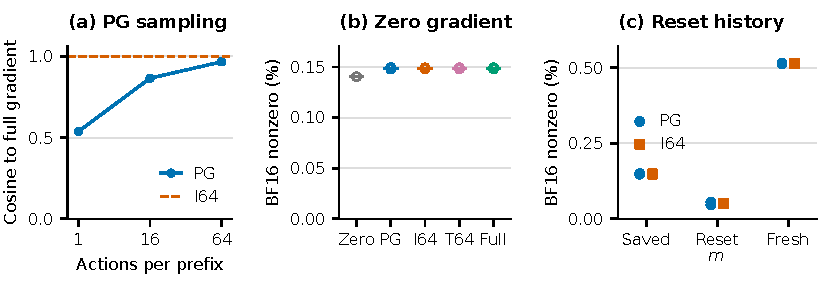
\includegraphics[width=\linewidth]{figures/added_control_figures_20260914/sampling_history_controls.pdf}
\caption{\textbf{Averaging more token samples improves gradient alignment; Adam history contributes strongly to BF16 changes.}
(a) Gradient cosine to full-vocabulary supervision as the number of sampled tokens per prefix increases; I64 uses the top-64 intersection.
(b,c) Fractions of changed BF16 weights with zero current gradient or reset moments. PG denotes sampled-token supervision; reset-$m$ keeps the second moment and step count, and fresh Adam resets both moments and the count. Points show batches and bars show means.}
\label{fig:sampling_history_controls}
\end{figure}
